% Options for packages loaded elsewhere
\PassOptionsToPackage{unicode}{hyperref}
\PassOptionsToPackage{hyphens}{url}
%
\documentclass[
]{article}
\usepackage{lmodern}
\usepackage{amssymb,amsmath}
\usepackage{ifxetex,ifluatex}
\ifnum 0\ifxetex 1\fi\ifluatex 1\fi=0 % if pdftex
  \usepackage[T1]{fontenc}
  \usepackage[utf8]{inputenc}
  \usepackage{textcomp} % provide euro and other symbols
\else % if luatex or xetex
  \usepackage{unicode-math}
  \defaultfontfeatures{Scale=MatchLowercase}
  \defaultfontfeatures[\rmfamily]{Ligatures=TeX,Scale=1}
\fi
% Use upquote if available, for straight quotes in verbatim environments
\IfFileExists{upquote.sty}{\usepackage{upquote}}{}
\IfFileExists{microtype.sty}{% use microtype if available
  \usepackage[]{microtype}
  \UseMicrotypeSet[protrusion]{basicmath} % disable protrusion for tt fonts
}{}
\makeatletter
\@ifundefined{KOMAClassName}{% if non-KOMA class
  \IfFileExists{parskip.sty}{%
    \usepackage{parskip}
  }{% else
    \setlength{\parindent}{0pt}
    \setlength{\parskip}{6pt plus 2pt minus 1pt}}
}{% if KOMA class
  \KOMAoptions{parskip=half}}
\makeatother
\usepackage{xcolor}
\IfFileExists{xurl.sty}{\usepackage{xurl}}{} % add URL line breaks if available
\IfFileExists{bookmark.sty}{\usepackage{bookmark}}{\usepackage{hyperref}}
\hypersetup{
  pdftitle={Reproducible Research: Peer Assessment 1},
  pdfauthor={rlfacanha},
  hidelinks,
  pdfcreator={LaTeX via pandoc}}
\urlstyle{same} % disable monospaced font for URLs
\usepackage[margin=1in]{geometry}
\usepackage{color}
\usepackage{fancyvrb}
\newcommand{\VerbBar}{|}
\newcommand{\VERB}{\Verb[commandchars=\\\{\}]}
\DefineVerbatimEnvironment{Highlighting}{Verbatim}{commandchars=\\\{\}}
% Add ',fontsize=\small' for more characters per line
\usepackage{framed}
\definecolor{shadecolor}{RGB}{248,248,248}
\newenvironment{Shaded}{\begin{snugshade}}{\end{snugshade}}
\newcommand{\AlertTok}[1]{\textcolor[rgb]{0.94,0.16,0.16}{#1}}
\newcommand{\AnnotationTok}[1]{\textcolor[rgb]{0.56,0.35,0.01}{\textbf{\textit{#1}}}}
\newcommand{\AttributeTok}[1]{\textcolor[rgb]{0.77,0.63,0.00}{#1}}
\newcommand{\BaseNTok}[1]{\textcolor[rgb]{0.00,0.00,0.81}{#1}}
\newcommand{\BuiltInTok}[1]{#1}
\newcommand{\CharTok}[1]{\textcolor[rgb]{0.31,0.60,0.02}{#1}}
\newcommand{\CommentTok}[1]{\textcolor[rgb]{0.56,0.35,0.01}{\textit{#1}}}
\newcommand{\CommentVarTok}[1]{\textcolor[rgb]{0.56,0.35,0.01}{\textbf{\textit{#1}}}}
\newcommand{\ConstantTok}[1]{\textcolor[rgb]{0.00,0.00,0.00}{#1}}
\newcommand{\ControlFlowTok}[1]{\textcolor[rgb]{0.13,0.29,0.53}{\textbf{#1}}}
\newcommand{\DataTypeTok}[1]{\textcolor[rgb]{0.13,0.29,0.53}{#1}}
\newcommand{\DecValTok}[1]{\textcolor[rgb]{0.00,0.00,0.81}{#1}}
\newcommand{\DocumentationTok}[1]{\textcolor[rgb]{0.56,0.35,0.01}{\textbf{\textit{#1}}}}
\newcommand{\ErrorTok}[1]{\textcolor[rgb]{0.64,0.00,0.00}{\textbf{#1}}}
\newcommand{\ExtensionTok}[1]{#1}
\newcommand{\FloatTok}[1]{\textcolor[rgb]{0.00,0.00,0.81}{#1}}
\newcommand{\FunctionTok}[1]{\textcolor[rgb]{0.00,0.00,0.00}{#1}}
\newcommand{\ImportTok}[1]{#1}
\newcommand{\InformationTok}[1]{\textcolor[rgb]{0.56,0.35,0.01}{\textbf{\textit{#1}}}}
\newcommand{\KeywordTok}[1]{\textcolor[rgb]{0.13,0.29,0.53}{\textbf{#1}}}
\newcommand{\NormalTok}[1]{#1}
\newcommand{\OperatorTok}[1]{\textcolor[rgb]{0.81,0.36,0.00}{\textbf{#1}}}
\newcommand{\OtherTok}[1]{\textcolor[rgb]{0.56,0.35,0.01}{#1}}
\newcommand{\PreprocessorTok}[1]{\textcolor[rgb]{0.56,0.35,0.01}{\textit{#1}}}
\newcommand{\RegionMarkerTok}[1]{#1}
\newcommand{\SpecialCharTok}[1]{\textcolor[rgb]{0.00,0.00,0.00}{#1}}
\newcommand{\SpecialStringTok}[1]{\textcolor[rgb]{0.31,0.60,0.02}{#1}}
\newcommand{\StringTok}[1]{\textcolor[rgb]{0.31,0.60,0.02}{#1}}
\newcommand{\VariableTok}[1]{\textcolor[rgb]{0.00,0.00,0.00}{#1}}
\newcommand{\VerbatimStringTok}[1]{\textcolor[rgb]{0.31,0.60,0.02}{#1}}
\newcommand{\WarningTok}[1]{\textcolor[rgb]{0.56,0.35,0.01}{\textbf{\textit{#1}}}}
\usepackage{graphicx,grffile}
\makeatletter
\def\maxwidth{\ifdim\Gin@nat@width>\linewidth\linewidth\else\Gin@nat@width\fi}
\def\maxheight{\ifdim\Gin@nat@height>\textheight\textheight\else\Gin@nat@height\fi}
\makeatother
% Scale images if necessary, so that they will not overflow the page
% margins by default, and it is still possible to overwrite the defaults
% using explicit options in \includegraphics[width, height, ...]{}
\setkeys{Gin}{width=\maxwidth,height=\maxheight,keepaspectratio}
% Set default figure placement to htbp
\makeatletter
\def\fps@figure{htbp}
\makeatother
\setlength{\emergencystretch}{3em} % prevent overfull lines
\providecommand{\tightlist}{%
  \setlength{\itemsep}{0pt}\setlength{\parskip}{0pt}}
\setcounter{secnumdepth}{-\maxdimen} % remove section numbering

\title{Reproducible Research: Peer Assessment 1}
\author{rlfacanha}
\date{17/08/2020}

\begin{document}
\maketitle

\hypertarget{loading-and-preprocessing-the-data}{%
\subsection{Loading and preprocessing the
data}\label{loading-and-preprocessing-the-data}}

\begin{Shaded}
\begin{Highlighting}[]
\KeywordTok{unzip}\NormalTok{(}\StringTok{"activity.zip"}\NormalTok{)}
\CommentTok{#Read dataset and load into data table object}
\NormalTok{activity <-}\StringTok{ }\KeywordTok{read.table}\NormalTok{(}\StringTok{"activity.csv"}\NormalTok{, }\DataTypeTok{sep =} \StringTok{","}\NormalTok{,}\DataTypeTok{header =} \OtherTok{TRUE}\NormalTok{)}
\end{Highlighting}
\end{Shaded}

\hypertarget{what-is-mean-total-number-of-steps-taken-per-day}{%
\subsection{What is mean total number of steps taken per
day?}\label{what-is-mean-total-number-of-steps-taken-per-day}}

\begin{Shaded}
\begin{Highlighting}[]
\KeywordTok{library}\NormalTok{(dplyr)}
\end{Highlighting}
\end{Shaded}

\begin{verbatim}
## 
## Attaching package: 'dplyr'
\end{verbatim}

\begin{verbatim}
## The following objects are masked from 'package:stats':
## 
##     filter, lag
\end{verbatim}

\begin{verbatim}
## The following objects are masked from 'package:base':
## 
##     intersect, setdiff, setequal, union
\end{verbatim}

\begin{Shaded}
\begin{Highlighting}[]
\CommentTok{#Ignoring missing values}
\NormalTok{activity_na <-}\StringTok{ }\NormalTok{activity[}\KeywordTok{complete.cases}\NormalTok{(activity), ]}
\CommentTok{#1. Calculate the total number of steps taken per day}
\NormalTok{totalsteps_perday <-}\StringTok{ }\NormalTok{activity_na }\OperatorTok\StringTok{ }\KeywordTok{group_by}\NormalTok{(date) }\OperatorTok\StringTok{ }\KeywordTok{summarize}\NormalTok{(}\DataTypeTok{totalsteps=}\KeywordTok{sum}\NormalTok{(steps))}
\end{Highlighting}
\end{Shaded}

\begin{verbatim}
## `summarise()` ungrouping output (override with `.groups` argument)
\end{verbatim}

\begin{Shaded}
\begin{Highlighting}[]
\CommentTok{#2. Make a histogram of the total number of steps taken each day}
\KeywordTok{hist}\NormalTok{(totalsteps_perday}\OperatorTok{$}\NormalTok{totalsteps, }\DataTypeTok{xlab =} \StringTok{"Total Steps Per Day"}\NormalTok{, }\DataTypeTok{col =} \StringTok{"red"}\NormalTok{, }\DataTypeTok{main =} \StringTok{"Histogram of the total number of steps taken each day"}\NormalTok{)}
\end{Highlighting}
\end{Shaded}

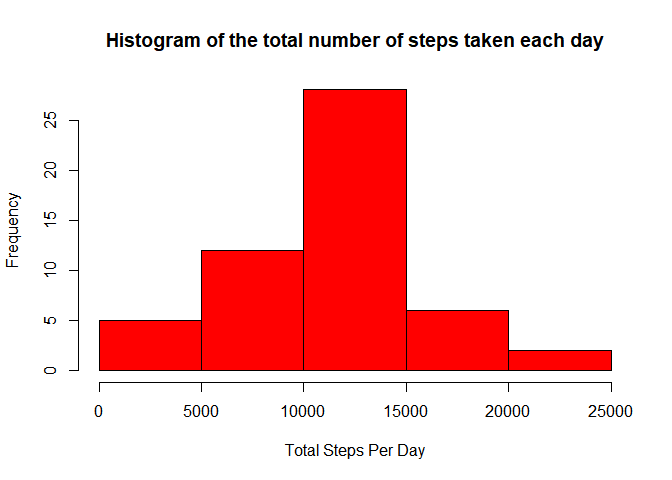
\includegraphics{PA1_template_files/figure-latex/activity_mean_steps-1.pdf}

\begin{Shaded}
\begin{Highlighting}[]
\KeywordTok{dev.copy}\NormalTok{(png, }\DataTypeTok{file =} \StringTok{"figures/plot_totalsteps_perday.png"}\NormalTok{)}
\end{Highlighting}
\end{Shaded}

png 3

\begin{Shaded}
\begin{Highlighting}[]
\KeywordTok{dev.off}\NormalTok{()}
\end{Highlighting}
\end{Shaded}

pdf 2

\begin{Shaded}
\begin{Highlighting}[]
\CommentTok{#3. Calculate and report the mean and median of the total number of steps taken per day}
\KeywordTok{mean}\NormalTok{(totalsteps_perday}\OperatorTok{$}\NormalTok{totalsteps)}
\end{Highlighting}
\end{Shaded}

{[}1{]} 10766.19

\begin{Shaded}
\begin{Highlighting}[]
\KeywordTok{median}\NormalTok{(totalsteps_perday}\OperatorTok{$}\NormalTok{totalsteps)}
\end{Highlighting}
\end{Shaded}

{[}1{]} 10765

\hypertarget{what-is-the-average-daily-activity-pattern}{%
\subsection{What is the average daily activity
pattern?}\label{what-is-the-average-daily-activity-pattern}}

\begin{Shaded}
\begin{Highlighting}[]
\CommentTok{#1. Make a time series plot (i.e. \textbackslash{}color\{red\}\{\textbackslash{}verb|type = "l"|\}type = "l") of the 5-minute interval (x-axis) and the average number of steps taken, averaged across all days (y-axis)}
\NormalTok{steps_per_interval <-}\StringTok{ }\NormalTok{activity_na }\OperatorTok\StringTok{ }\KeywordTok{group_by}\NormalTok{(interval) }\OperatorTok\StringTok{ }\KeywordTok{summarise}\NormalTok{(}\DataTypeTok{avgsteps =} \KeywordTok{mean}\NormalTok{(steps, }\DataTypeTok{na.rm=}\OtherTok{TRUE}\NormalTok{))}
\end{Highlighting}
\end{Shaded}

\begin{verbatim}
## `summarise()` ungrouping output (override with `.groups` argument)
\end{verbatim}

\begin{Shaded}
\begin{Highlighting}[]
\KeywordTok{plot}\NormalTok{(steps_per_interval}\OperatorTok{$}\NormalTok{interval,}
\NormalTok{                             steps_per_interval}\OperatorTok{$}\NormalTok{avgsteps, }
                             \DataTypeTok{xlab =} \StringTok{"5-minute interval"}\NormalTok{,}
                             \DataTypeTok{ylab =} \StringTok{"Average Number of Steps"}\NormalTok{,             }
                             \DataTypeTok{type=}\StringTok{'l'}\NormalTok{,}
                             \DataTypeTok{main =} \StringTok{"Time Series of steps by 5 minute interval"}\NormalTok{)}
\end{Highlighting}
\end{Shaded}

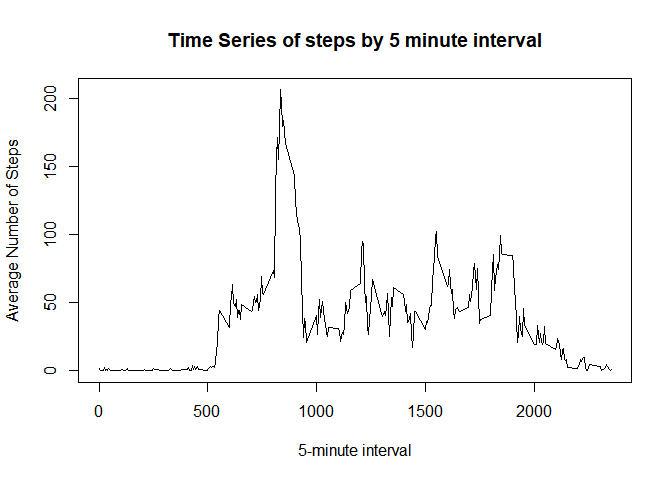
\includegraphics{PA1_template_files/figure-latex/daily_activity_pattern-1.pdf}

\begin{Shaded}
\begin{Highlighting}[]
\KeywordTok{dev.copy}\NormalTok{(png, }\DataTypeTok{file =} \StringTok{"figures/plot_steps_per_interval.png"}\NormalTok{)}
\end{Highlighting}
\end{Shaded}

png 3

\begin{Shaded}
\begin{Highlighting}[]
\KeywordTok{dev.off}\NormalTok{()}
\end{Highlighting}
\end{Shaded}

pdf 2

\begin{Shaded}
\begin{Highlighting}[]
\CommentTok{#2. Which 5-minute interval, on average across all the days in the dataset, contains the maximum number of steps?}
\CommentTok{#steps_per_interval[which.max(steps_per_interval$avgsteps),]}
\KeywordTok{print}\NormalTok{(}\KeywordTok{paste}\NormalTok{(}\StringTok{"Interval: "}\NormalTok{, steps_per_interval[}\KeywordTok{which.max}\NormalTok{(steps_per_interval}\OperatorTok{$}\NormalTok{avgsteps),][}\DecValTok{1}\NormalTok{]))}
\end{Highlighting}
\end{Shaded}

{[}1{]} ``Interval: 835''

\hypertarget{imputing-missing-values}{%
\subsection{Imputing missing values}\label{imputing-missing-values}}

\begin{Shaded}
\begin{Highlighting}[]
\CommentTok{#1. Calculate and report the total number of missing values in the dataset (i.e. the total number of rows with \textbackslash{}color\{red\}\{\textbackslash{}verb|NA|\}NAs)}
\KeywordTok{print}\NormalTok{(}\KeywordTok{paste}\NormalTok{(}\StringTok{"Number of missing values: "}\NormalTok{, }\KeywordTok{sum}\NormalTok{(}\KeywordTok{is.na}\NormalTok{(activity))))}
\end{Highlighting}
\end{Shaded}

{[}1{]} ``Number of missing values: 2304''

\begin{Shaded}
\begin{Highlighting}[]
\CommentTok{#2. Devise a strategy for filling in all of the missing values in the dataset. The strategy does not need to be sophisticated. For example, you could use the mean/median for that day, or the mean for that 5-minute interval, etc.}
\KeywordTok{print}\NormalTok{(}\StringTok{"The strategy will fill the NA values with the number of steps corresponding the mean for the corresponding 5-minute interval."}\NormalTok{)}
\end{Highlighting}
\end{Shaded}

{[}1{]} ``The strategy will fill the NA values with the number of steps
corresponding the mean for the corresponding 5-minute interval.''

\begin{Shaded}
\begin{Highlighting}[]
\CommentTok{#3. Create a new dataset that is equal to the original dataset but with the missing data filled in.}
\NormalTok{filled_activity <-}\StringTok{ }\NormalTok{activity}
\ControlFlowTok{for}\NormalTok{ (row }\ControlFlowTok{in} \DecValTok{1}\OperatorTok{:}\KeywordTok{nrow}\NormalTok{(activity)) \{}
        \ControlFlowTok{if}\NormalTok{ (}\KeywordTok{is.na}\NormalTok{(activity}\OperatorTok{$}\NormalTok{steps[row])) \{}
\NormalTok{                steps_to_fill <-}\StringTok{ }\NormalTok{steps_per_interval}\OperatorTok{$}\NormalTok{avgsteps[steps_per_interval}\OperatorTok{$}\NormalTok{interval }\OperatorTok{==}\StringTok{ }\NormalTok{activity}\OperatorTok{$}\NormalTok{interval[row]]}
\NormalTok{                filled_activity}\OperatorTok{$}\NormalTok{steps[row] <-}\StringTok{ }\NormalTok{steps_to_fill}
\NormalTok{        \}        }
\NormalTok{\}}
\CommentTok{#4. Make a histogram of the total number of steps taken each day and Calculate and report the mean and median total number of steps taken per day. Do these values differ from the estimates from the first part of the assignment? What is the impact of imputing missing data on the estimates of the total daily number of steps?}
\NormalTok{filled_totalsteps_perday <-}\StringTok{ }\NormalTok{filled_activity }\OperatorTok\StringTok{ }\KeywordTok{group_by}\NormalTok{(date) }\OperatorTok\StringTok{ }\KeywordTok{summarize}\NormalTok{(}\DataTypeTok{totalsteps=}\KeywordTok{sum}\NormalTok{(steps))}
\end{Highlighting}
\end{Shaded}

\begin{verbatim}
## `summarise()` ungrouping output (override with `.groups` argument)
\end{verbatim}

\begin{Shaded}
\begin{Highlighting}[]
\KeywordTok{hist}\NormalTok{(filled_totalsteps_perday}\OperatorTok{$}\NormalTok{totalsteps, }
          \DataTypeTok{xlab =} \StringTok{"Total Steps Per Day"}\NormalTok{, }\DataTypeTok{col =} \StringTok{"red"}\NormalTok{, }
          \DataTypeTok{main =} \StringTok{"Histogram of the total number of steps taken each day"}\NormalTok{)}
\end{Highlighting}
\end{Shaded}

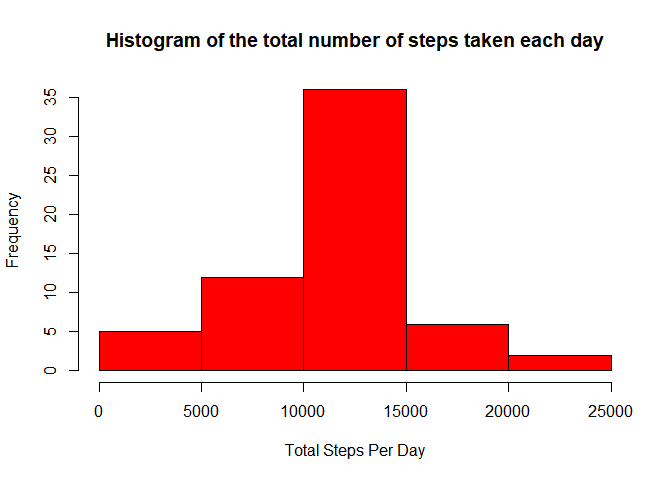
\includegraphics{PA1_template_files/figure-latex/missing_values-1.pdf}

\begin{Shaded}
\begin{Highlighting}[]
\KeywordTok{dev.copy}\NormalTok{(png, }\DataTypeTok{file =} \StringTok{"figures/filled_totalsteps_perday.png"}\NormalTok{)}
\end{Highlighting}
\end{Shaded}

png 3

\begin{Shaded}
\begin{Highlighting}[]
\KeywordTok{dev.off}\NormalTok{()}
\end{Highlighting}
\end{Shaded}

pdf 2

\begin{Shaded}
\begin{Highlighting}[]
\KeywordTok{mean}\NormalTok{(filled_totalsteps_perday}\OperatorTok{$}\NormalTok{totalsteps)}
\end{Highlighting}
\end{Shaded}

{[}1{]} 10766.19

\begin{Shaded}
\begin{Highlighting}[]
\KeywordTok{median}\NormalTok{(filled_totalsteps_perday}\OperatorTok{$}\NormalTok{totalsteps)}
\end{Highlighting}
\end{Shaded}

{[}1{]} 10766.19

\begin{Shaded}
\begin{Highlighting}[]
\KeywordTok{print}\NormalTok{(}\StringTok{"The mean value does not differ and the median differs just slightly. The impact depends on the devised strategy"}\NormalTok{)}
\end{Highlighting}
\end{Shaded}

{[}1{]} ``The mean value does not differ and the median differs just
slightly. The impact depends on the devised strategy''

\hypertarget{are-there-differences-in-activity-patterns-between-weekdays-and-weekends}{%
\subsection{Are there differences in activity patterns between weekdays
and
weekends?}\label{are-there-differences-in-activity-patterns-between-weekdays-and-weekends}}

\begin{Shaded}
\begin{Highlighting}[]
\CommentTok{#1. Create a new factor variable in the dataset with two levels – “weekday” and “weekend” indicating whether a given date is a weekday or weekend day.}
\NormalTok{weekdays_weekday <-}\StringTok{ }\KeywordTok{c}\NormalTok{(}\StringTok{"segunda-feira"}\NormalTok{,}\StringTok{"terça-feira"}\NormalTok{,}\StringTok{"quarta-feira"}\NormalTok{,}\StringTok{"quinta-feira"}\NormalTok{,}\StringTok{"sexta-feira"}\NormalTok{)}
\NormalTok{filled_activity}\OperatorTok{$}\NormalTok{wDay <-}\StringTok{ }\KeywordTok{c}\NormalTok{(}\StringTok{'weekend'}\NormalTok{, }\StringTok{'weekday'}\NormalTok{)[(}\KeywordTok{weekdays}\NormalTok{(}\KeywordTok{as.Date}\NormalTok{(activity}\OperatorTok{$}\NormalTok{date)) }\OperatorTok\StringTok{ }\NormalTok{weekdays_weekday)}\OperatorTok{+}\NormalTok{1L]}
\CommentTok{#2. Make a panel plot containing a time series plot (i.e. \textbackslash{}color\{red\}\{\textbackslash{}verb|type = "l"|\}type = "l") of the 5-minute interval (x-axis) and the average number of steps taken, averaged across all weekday days or weekend days (y-axis). See the README file in the GitHub repository to see an example of what this plot should look like using simulated data.}
\KeywordTok{library}\NormalTok{(ggplot2)}
\NormalTok{steps_perweekday <-}\StringTok{ }\NormalTok{filled_activity }\OperatorTok\StringTok{ }\KeywordTok{group_by}\NormalTok{(interval,wDay) }\OperatorTok\StringTok{ }\KeywordTok{summarise}\NormalTok{(}\DataTypeTok{avgsteps =} \KeywordTok{mean}\NormalTok{(steps, }\DataTypeTok{na.rm=}\OtherTok{TRUE}\NormalTok{))}
\end{Highlighting}
\end{Shaded}

\begin{verbatim}
## `summarise()` regrouping output by 'interval' (override with `.groups` argument)
\end{verbatim}

\begin{Shaded}
\begin{Highlighting}[]
\KeywordTok{qplot}\NormalTok{(interval, avgsteps, }\DataTypeTok{data=}\NormalTok{steps_perweekday,}
                \DataTypeTok{xlab =} \StringTok{"5-minute interval"}\NormalTok{,}
                \DataTypeTok{ylab =} \StringTok{"Average Number of Steps"}\NormalTok{,                }
                \DataTypeTok{geom=}\StringTok{"line"}\NormalTok{,}
                \DataTypeTok{main =} \StringTok{"Time Series of steps by 5 minute interval and weekend/weekday"}\NormalTok{,}
                \DataTypeTok{facets =}\NormalTok{ wDay }\OperatorTok{~}\StringTok{ }\NormalTok{.)}
\end{Highlighting}
\end{Shaded}

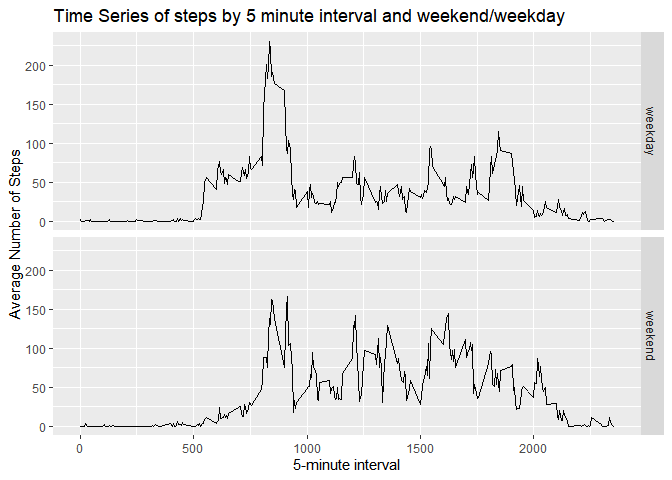
\includegraphics{PA1_template_files/figure-latex/weekdays-1.pdf}

\begin{Shaded}
\begin{Highlighting}[]
\KeywordTok{dev.copy}\NormalTok{(png, }\DataTypeTok{file =} \StringTok{"figures/steps_perweekday.png"}\NormalTok{)}
\end{Highlighting}
\end{Shaded}

png 3

\begin{Shaded}
\begin{Highlighting}[]
\KeywordTok{dev.off}\NormalTok{()}
\end{Highlighting}
\end{Shaded}

pdf 2

\end{document}
